% Provenance (never printed): old terminale S material on absolute dating (the
% decay law recalled, the closed system, the rubidium-strontium isochron) and on
% the history of the age of the Earth (cooling, salt, sediments, then radioactivity,
% meteorites and 4.55 billion years). Owner (Sync 0/1): closed system, isochron,
% age of the Earth (as a defined notion). The decay law, the half-life and the
% dating equation are the physics books' (recalled); relative dating, absolute
% age, superposition, cross-cutting relationships and the eras are Book 1 g7's
% (recalled); the oldest zircons and the Acasta gneiss are g12.01's (quoted).
% Varden Hills granite 310 Ma and schist 480 Ma from figdata/shared/region.py;
% their isotope ratios are exercise data (figdata/grade-12/isochrons.py).
\chapter{放射性测年与地球年龄}\label{ch:g12:age-of-the-earth}

1862 年，物理学家威廉·汤姆孙（后来的开尔文勋爵）
根据地球的冷却过程推算地球的年龄。他假定地球起初是熔融的，此后一直在散失热量，
并问地表附近的温度梯度降到现在的数值需要多长时间。
他的答案是 9600 万年，
介于 2000 万至 4 亿年之间；
到 1897 年，他把范围缩小到 2000 万至 4000 万年。
地质学家发现，这一数字远远短于岩石中记录的历史。
答案来自放射性，而开尔文当时并不知道放射性。
% ledger: holmes13:estimates, england:kelvin (Book 3 row)

\begin{omfigure}
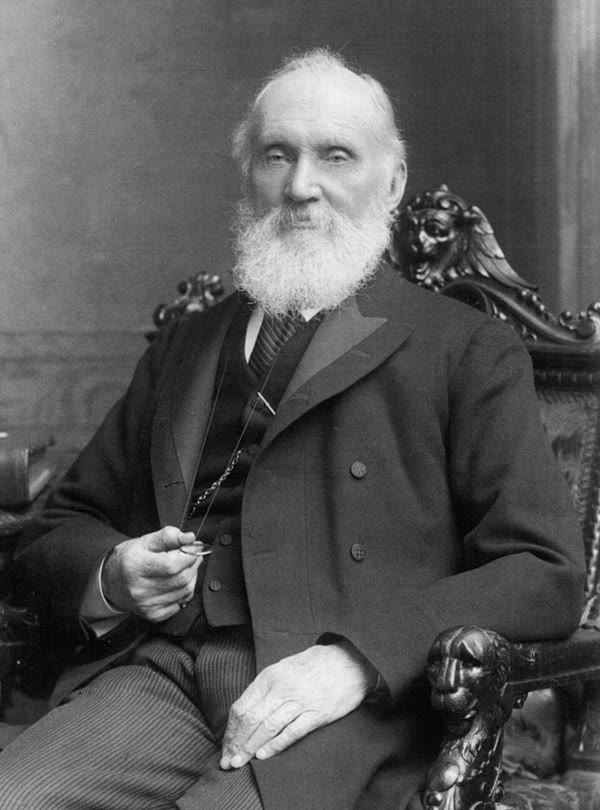
\includegraphics[height=5.2cm]{images/book2/g12-kelvin-1906.jpg}

{\small 威廉·汤姆孙，即开尔文勋爵，摄于 1906 年。照片由罗素父子公司拍摄，
伦敦（Smithsonian Institution Libraries，无已知版权限制）。}
\end{omfigure}
% ledger: photo:g12-kelvin

\begin{recall}
相对定年用于确定岩石和事件的先后顺序，绝对年龄则是一个以年计的数值
（第 1 册，七年级）。放射性同位素（即母体）
随机地衰变为子体同位素：剩余母体原子数 $N$ 按
$N = N_0\,e^{-\lambda t}$ 规律递减，其中 $\lambda$ 为衰变常数，
每经过一个半衰期 $T = \ln 2/\lambda$ 减半（见物理教材）。已知最古老的矿物
是产自西澳大利亚的锆石，其年龄为 44 亿年
（见\cref{ch:g12:continental-crust}）。地球还在散失放射性持续产生的热量，
地幔也在对流（见\cref{ch:g12:internal-heat}）。
\end{recall}
% ledger: wilde01:zircon

\section{历次估算}

在放射性被发现之前，每一种\omterm{def:g12:age-of-the-earth:age}{地球年龄}的估算，
都依赖于一个速率被认为已知的过程。

\begin{center}
\small
\begin{tabular}{|p{0.19\linewidth}|p{0.42\linewidth}|p{0.25\linewidth}|}
\hline
谁、何时 & 方法及其假设 & 估算值 \\
\hline
菲利普斯，1860 年 & 沉积层的厚度除以沉积速率；假设沉积速率恒定 & 3800 万至 9600 万年 \\
开尔文，1862 年 & 仅由传导使熔融地球冷却，内部没有热源 & 2000 万至 4 亿年 \\
G.\,H.~达尔文 & 月球与地球分离以来的时间，由潮汐使两者运动减慢推算 & 至少 5600 万年 \\
约利，1899 年 & 河流带入海洋的盐量除以每年的输入量；假设输入量恒定且盐不被移除 & 8000 万至 1 亿年 \\
\hline
\end{tabular}
\end{center}
% ledger: holmes13:estimates

\begin{history}[开尔文缺失的热量]
1903 年，皮埃尔·居里和阿尔伯特·拉博德证明镭会放出热量，
一些科学家随即认为，这种热量推翻了开尔文的结论。
一年后，欧内斯特·卢瑟福在讲座上，开尔文在台下听讲，
卢瑟福提醒他，开尔文曾把\omterm{def:g12:age-of-the-earth:age}{地球年龄}限定在
“在没有发现新的热源”的前提之下。放射性似乎就是那种热源。
然而这并不是开尔文的主要错误，真正最能延长地球冷却时间的是
\omterm{def:g12:internal-heat:convection}{地幔对流}，它使上地幔保持高温，并使地壳中的温度梯度在很长时间内保持较高，
远远长于仅靠传导所能维持的时间。
\end{history}
% ledger: england:kelvin (Book 3 row)

放射性还提供了一把“时钟”。1907 年，伯特伦·博尔特伍德证明，
年代相同的铀矿物，每克铀所含的铅量相同，
即铅是由铀产生的。1913 年，阿瑟·霍姆斯写道，
已测定的最古老岩石的年龄为 16 亿年。1927 年，他
将\omterm{def:g12:age-of-the-earth:age}{地球年龄}估计在 16 亿至 30 亿年之间。1956 年，克莱尔·帕特森
测得 45.5 亿年。现今的值为 45.4 亿年，
误差在百分之一以内。
% ledger: holmes13:estimates, holmes27:age, patterson56:table, usgs:age-earth (Book 1 row)

\begin{omfigure}
\begin{tikzpicture}
\begin{axis}[omrecord, width=0.78\linewidth, height=6.2cm, ymode=log, xmin=1840, xmax=2040,
  ymin=1e7, ymax=2e10, xlabel={估算年份}, ylabel={地球的估计年龄（年）},
  xtick={1850,1875,...,2025}, x tick label style={/pgf/number format/.cd, set thousands separator={}},
  ytick={1e7,1e8,1e9,1e10}, ymajorgrids=true, xmajorgrids=false]
% computed in figdata/grade-12/isochrons.py; ledger: holmes13:estimates, holmes27:age, patterson56:table, usgs:age-earth (Book 1 row)
\addplot[omDef, only marks, mark=*, mark size=1.8pt, error bars/.cd, y dir=both, y explicit]
  table[x=year, y=mid, y error minus expr=\thisrow{mid}-\thisrow{lo}, y error plus expr=\thisrow{hi}-\thisrow{mid}]
  {figdata/out/grade-12-isochrons-history.dat};
\addplot[omThm, densely dashed, domain=1840:2040, samples=2] {4.54e9};
\coordinate (k62) at (axis cs:1862,2.4e8);
\coordinate (k97) at (axis cs:1897,2.8e7);
\coordinate (jol) at (axis cs:1899,1e8);
\coordinate (h11) at (axis cs:1919,1.3e9);
\coordinate (pat) at (axis cs:1956,4.55e9);
\coordinate (now) at (axis cs:1845,4.54e9);
\end{axis}
\node[font=\scriptsize, anchor=west] at ([xshift=4pt]k62) {开尔文 1862};
\node[font=\scriptsize, anchor=east] at ([xshift=-4pt]k97) {开尔文 1897};
\node[font=\scriptsize, anchor=west] at ([xshift=4pt]jol) {约利};
\node[font=\scriptsize, anchor=north] at (h11) {霍姆斯};
\node[font=\scriptsize, anchor=north west] at ([xshift=2pt, yshift=-3pt]pat) {帕特森};
\node[font=\scriptsize, text=omThm, anchor=south west] at (now) {现今，45.4 亿年};
\end{tikzpicture}

{\small \omterm{def:g12:age-of-the-earth:age}{地球年龄}估算值随估算年份变化，采用对数刻度；
竖线表示各作者给出的范围。霍姆斯 1913 年的数据点
为当时测定的最古老岩石的年龄，是一个下限。资料来源：霍姆斯
（1913，1927）；帕特森（1956）；美国地质调查局。}
\end{omfigure}

\section{放射性时钟}

放射性时钟只有在开始计时以来
没有任何物质被加入或移\omterm{def:g11:seismic-structure:travel-time}{走时}才有效。

\begin{definition}[封闭系统]\label{def:g12:age-of-the-earth:closed-system}
岩石或矿物对母同位素及其子体而言，若是\emph{封闭系统}\index{封闭系统}，
即自计时开始的时刻起，
除母体衰变为子体的过程外，母体或子体的原子
未曾进入或离开该岩石或矿物。
\end{definition}
% ledger: tulane:radiometric

对于矿物，计时始于其从岩浆中结晶之时，或更确切地说，
即其冷却至原子不再进出它的程度之时。
加热、\omterm{def:g12:internal-heat:heat-flow}{热流}体或风化可使系统重新开放，
此时所测得的年龄
是错误的，或测定的是后来那一事件的年代。
% ledger: tulane:radiometric

在\omterm{def:g12:age-of-the-earth:closed-system}{封闭系统}中，计数子体原子即可得出年龄，前提是
已知开始时有多少。通常并不知道。铷-87
衰变为锶-87，但每种矿物在形成时也
吸收了一些锶-87。\omterm{def:g12:age-of-the-earth:isochron}{等时线}方法通过测量同一岩石的几种矿物
来绕过这一问题。

\section{等时线}

锶有一种同位素锶-86，它是稳定的，
不由任何衰变产生：在\omterm{def:g12:age-of-the-earth:closed-system}{封闭系统}中其数目保持不变，可作为
参照标尺。同位素比 $^{87}\mathrm{Sr}/^{86}\mathrm{Sr}$ 和
$^{87}\mathrm{Rb}/^{86}\mathrm{Sr}$ 是质谱仪测得的量。

\begin{theorem}[等时线方程]\label{thm:g12:age-of-the-earth:isochron}
对于在时间 $t$ 内一直为\omterm{def:g12:age-of-the-earth:closed-system}{封闭系统}的矿物，
\[
  \left(\frac{^{87}\mathrm{Sr}}{^{86}\mathrm{Sr}}\right)_{\text{现在}}
  = \left(\frac{^{87}\mathrm{Sr}}{^{86}\mathrm{Sr}}\right)_{0}
  + \left(\frac{^{87}\mathrm{Rb}}{^{86}\mathrm{Sr}}\right)_{\text{现在}}
  \left(e^{\lambda t} - 1\right),
\]
其中下标 0 表示计时开始时的值，$\lambda$ 为
铷-87 的衰变常数。
\end{theorem}

\begin{proof}
设 $P$ 为现在铷-87 原子的数目，$P_0$ 为
计时开始时的数目。由衰变律 $P = P_0\,e^{-\lambda t}$，于是 $P_0 = P\,e^{\lambda t}$，
则已衰变的原子数为 $P_0 - P = P\,(e^{\lambda t}-1)$。
在\omterm{def:g12:age-of-the-earth:closed-system}{封闭系统}中，每个已衰变的原子都变为一个锶-87 原子，
它与开始时已有的 $D_0$ 个原子相加：$D = D_0 + P\,(e^{\lambda
t}-1)$。两边除以未变的锶-86 原子数，
即得上述方程。
\end{proof}
% ledger: tulane:radiometric

同一花岗岩中的矿物结晶于同一岩浆，因此它们开始时
具有相同的比值 $(^{87}\mathrm{Sr}/^{86}\mathrm{Sr})_0$，但它们吸收的
铷的量差别很大。它们都具有相同的 $t$ 和相同的初始比值，因此
方程表明它们的数据点位于同一直线上。

\begin{definition}[等时线]\label{def:g12:age-of-the-earth:isochron}
\emph{等时线}\index{等时线}是这样一条直线，直线上的点
对应于在同一时间由同一来源形成、
且此后一直为\omterm{def:g12:age-of-the-earth:closed-system}{封闭系统}的矿物或岩石，
其纵坐标为子体与稳定同位素之比，
横坐标为母体与稳定同位素之比。其斜率
给出它们的年龄，直线与纵轴的交点给出它们的开始比值。
\end{definition}
% ledger: tulane:radiometric

\begin{proposition}[由斜率求年龄]\label{prop:g12:age-of-the-earth:slope}
若\omterm{def:g12:age-of-the-earth:isochron}{等时线}的斜率为 $m$，则年龄为
\[
  t = \frac{\ln(1+m)}{\lambda}.
\]
\end{proposition}

\begin{proof}
与\omterm{def:g12:age-of-the-earth:isochron}{等时线}方程比较可得 $m = e^{\lambda t} - 1$，
于是 $e^{\lambda t} = 1 + m$，$\lambda t = \ln(1+m)$，$t = \ln(1+m)/\lambda$。
\end{proof}

对于铷-87，$\lambda = \num{1.3972e-11}$ 每年，半衰期为
$\ln 2/\lambda \approx 49.6$ 亿年，超过
\omterm{def:g12:age-of-the-earth:age}{地球年龄}的十倍以上。
% ledger: villa22:rb87

\begin{method}[用等时线给岩石定年]\label{met:g12:age-of-the-earth:isochron}
\begin{enumerate}
  \item 分离出该岩石中含铷量不同的几种矿物
        （或取该岩石的几个样品）。
  \item 测量每个样品的比值 $^{87}\mathrm{Rb}/^{86}\mathrm{Sr}$（$x$）
        和 $^{87}\mathrm{Sr}/^{86}\mathrm{Sr}$（$y$）。
  \item 以 $y$ 对 $x$ 作图，检验各点是否位于一条直线上；
        若不在，则该样品不是\omterm{def:g12:age-of-the-earth:closed-system}{封闭系统}。
  \item 求直线的斜率 $m$，并计算 $t = \ln(1+m)/\lambda$。
  \item 读出直线与纵轴交点处的开始比值。
\end{enumerate}
\end{method}

\begin{example}[瓦尔登花岗岩]\label{ex:g12:age-of-the-earth:varden}
瓦尔登丘陵的花岗岩，即本系列虚构的地区，给出以下
比值（练习数据）：
\begin{center}
\small
\begin{tabular}{|l|c|c|}
\hline
样品 & $^{87}\mathrm{Rb}/^{86}\mathrm{Sr}$ & $^{87}\mathrm{Sr}/^{86}\mathrm{Sr}$ \\
\hline
斜长石 & 0.35 & 0.70952 \\
角闪石  & 1.20 & 0.71321 \\
全岩  & 3.10 & 0.72146 \\
钾长石  & 6.40 & 0.73578 \\
黑云母     & 24.0 & 0.81218 \\
\hline
\end{tabular}
\end{center}
过斜长石与黑云母两点的直线斜率为
$m = (0.81218 - 0.70952)/(24.0 - 0.35) \approx 0.004341$。然后
$t = \ln(1.004341)/\num{1.3972e-11} \approx \num{3.10e8}$ 年：
该花岗岩的年龄为 3.1 亿年。直线与纵轴相交于
$0.70952 - 0.35 \times 0.004341 \approx 0.7080$，即开始比值。
\end{example}
% values: granite_age_Ma 310.0, granite_intercept 0.70800 (isochrons.py)

\begin{omfigure}
\begin{tikzpicture}
\begin{axis}[omrecord, width=0.7\linewidth, height=6cm, xmin=0, xmax=26, ymin=0.695, ymax=0.82, ytick={0.70,0.72,...,0.82},
  xlabel={$^{87}\mathrm{Rb}/^{86}\mathrm{Sr}$}, ylabel={$^{87}\mathrm{Sr}/^{86}\mathrm{Sr}$},
  y tick label style={/pgf/number format/.cd, fixed, fixed zerofill, precision=2}]
% computed in figdata/grade-12/isochrons.py (exercise data, Varden granite 310 Ma); ledger: villa22:rb87
\addplot[omDef, line width=0.9pt] table[x=x, y=y] {figdata/out/grade-12-isochrons-graniteln.dat};
\addplot[omThm, only marks, mark=*, mark size=2pt] table[x=rbsr, y=srsr] {figdata/out/grade-12-isochrons-granite.dat};
\addplot[black!60, densely dotted, domain=0:26, samples=2] {0.7080};
\coordinate (pl) at (axis cs:0.35,0.70952);
\coordinate (hb) at (axis cs:1.2,0.71321);
\coordinate (wr) at (axis cs:3.1,0.72146);
\coordinate (kf) at (axis cs:6.4,0.73578);
\coordinate (bt) at (axis cs:24,0.81218);
\coordinate (sl) at (axis cs:12,0.762);
\coordinate (in) at (axis cs:9,0.7082);
\coordinate (plhb) at (axis cs:0.6,0.737);
\coordinate (plhbpt) at (axis cs:0.9,0.7125);
\end{axis}
\node[font=\scriptsize, anchor=north west] at ([xshift=1pt]wr) {全岩};
\node[font=\scriptsize, anchor=north west] at ([xshift=1pt]kf) {钾长石};
\node[font=\scriptsize, anchor=east] at ([xshift=-3pt]bt) {黑云母};
\node[font=\scriptsize, anchor=south west, align=left, inner sep=1pt] (plhblab) at (plhb) {斜长石、\\角闪石};
\draw[black!60, line width=0.4pt] (plhblab.south) -- (plhbpt);
\node[font=\scriptsize, text=omDef, anchor=south east] at (sl) {斜率 $0.004341$：3.1 亿年};
\node[font=\scriptsize, text=black!70, anchor=south west] at (in) {开始比值 0.7080（时间 0）};
\end{tikzpicture}

{\small 瓦尔登花岗岩的铷–锶\omterm{def:g12:age-of-the-earth:isochron}{等时线}（练习
数据）。花岗岩形成时，所有矿物都位于水平的虚线上；
此后，每种矿物都按其铷含量的比例上升，
现在位于实线上。}
\end{omfigure}

\begin{inthelab}[称量原子]
比值用质谱仪测得。取几毫克矿物，溶于酸中，
再用化学方法将锶与铷分离，
因为两种质量数为 87 的同位素若不分离，
就会被一并计数。锶沉积在金属灯丝上，
在真空中加热后释放出离子；电场使离子加速，磁铁使其轨迹偏转，
较轻的离子偏转得比较重的离子更多，以使每种
同位素都到达各自的收集器。它们的电流给出比值。
\end{inthelab}

\begin{omfigure}
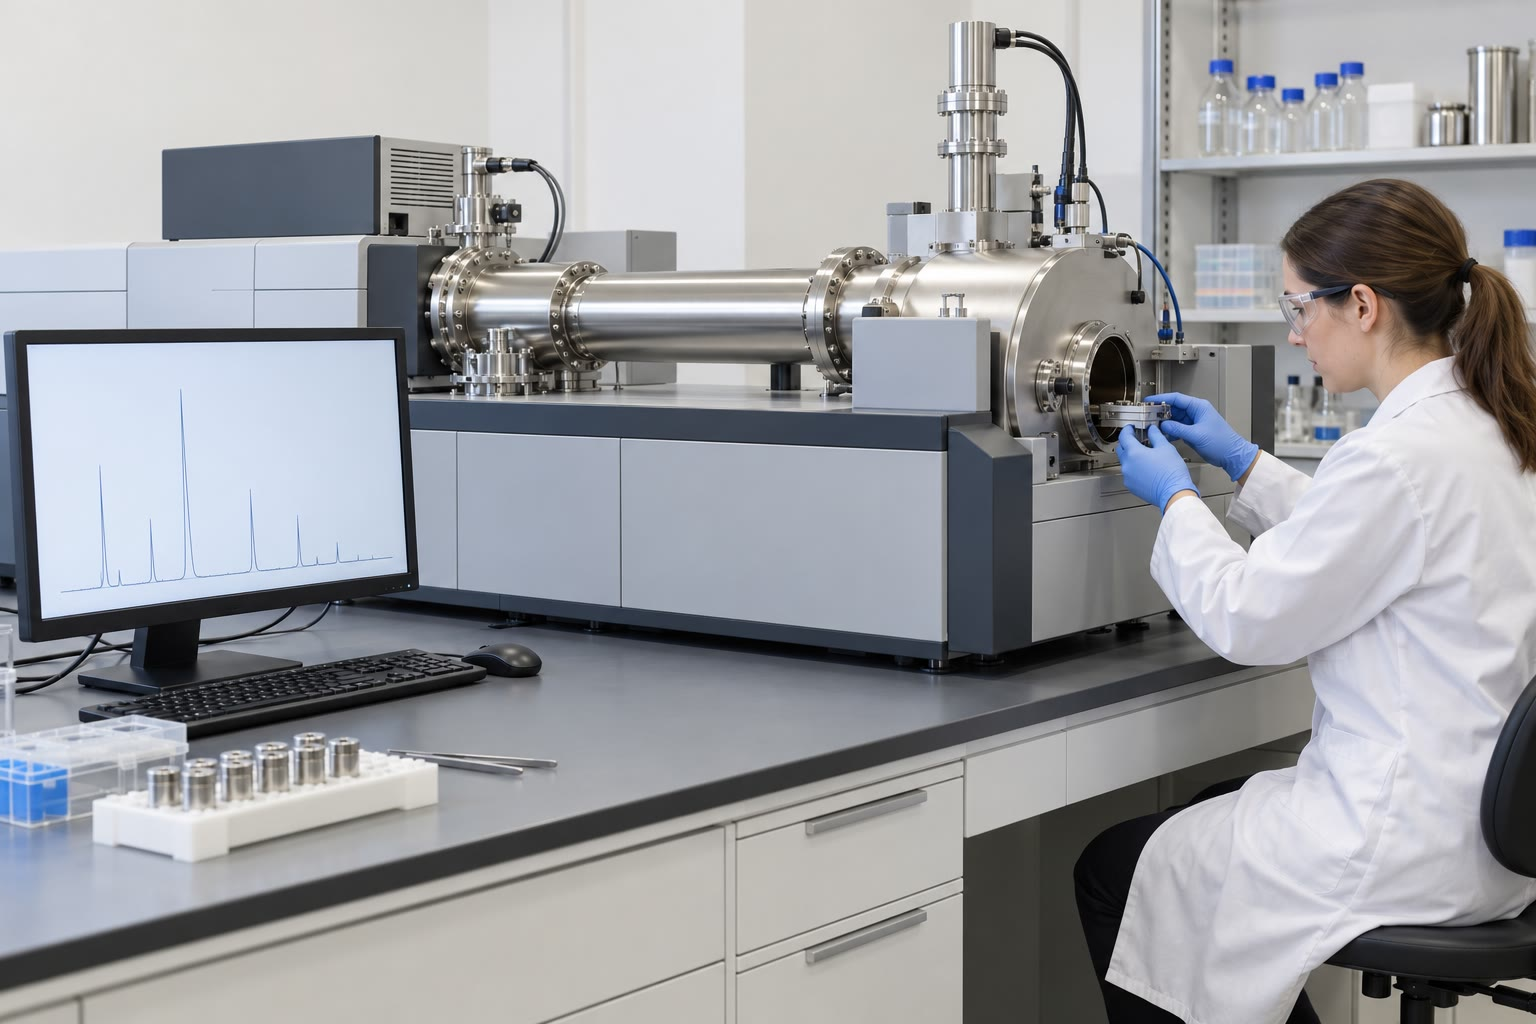
\includegraphics[width=0.66\linewidth]{images/book2/ai/g12-mass-spectrometer-lab.jpg}

{\small 实验室中的质谱仪：样品正在
源端装载。AI 生成的插图。}
\end{omfigure}

开始比值也是岩浆来源的线索。铷在地幔熔融时
更倾向于进入熔体，因此经过漫长岁月，它
富集于陆壳中，于是陆壳产生了更多
锶-87：地壳岩石的 $^{87}\mathrm{Sr}/^{86}\mathrm{Sr}$ 比高于
地幔岩石。由熔融地壳形成的岩浆继承了这一较高的比值。
% ledger: tulane:radiometric

\section{地球的年龄}

地球上没有任何岩石能追溯到地球形成之初：已知最古老的岩石，
阿卡斯塔片麻岩，年龄为 40.3 亿年，最古老的锆石为
44 亿年。此后地表多次被熔融、侵蚀和再循环。
地球本身的年龄来自陨石。陨石是与行星一同形成的小天体
的碎片，其中一些自那时起
便一直是\omterm{def:g12:age-of-the-earth:closed-system}{封闭系统}。
% ledger: bowring99:acasta, wilde01:zircon, usgs:age-earth (Book 1 row)

\begin{definition}[地球年龄]\label{def:g12:age-of-the-earth:age}
\emph{地球年龄}\index{地球年龄}是自地球由较小天体吸积形成以来
所经历的时间，起算点为太阳系诞生之时。
由陨石经放射性定年测得，其值为
\num{4.54}~十亿年，误差在百分之一以内。
\end{definition}
% ledger: usgs:age-earth (Book 1 row)

1956 年，克莱尔·帕特森测定了三块石陨石
和两块铁陨石中的铅同位素。其中两种由铀衰变生成，
铅-206 来自铀-238，铅-207 来自铀-235，
而铅-204 不由任何衰变生成。与锶的情形相似，陨石的数据点
若形成于同一时期，则落在一条直线上。作图时，
以 $^{207}\mathrm{Pb}/^{204}\mathrm{Pb}$ 为纵坐标、
$^{206}\mathrm{Pb}/^{204}\mathrm{Pb}$ 为横坐标。位于亚利桑那州的迪亚布洛峡谷铁陨石
几乎不含铀：其铅自形成以来未曾改变，
它标出了这条直线的下端，代表太阳系最初的铅。
% ledger: patterson56:table, patterson56:constants, usgs:age-earth (Book 1 row: Canyon Diablo troilite)

\begin{omfigure}
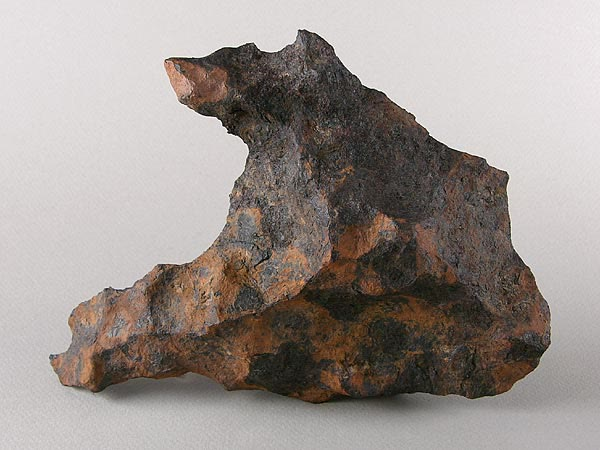
\includegraphics[height=4.2cm]{images/book2/g12-canyon-diablo-meteorite.jpg}

{\small 迪亚布洛峡谷铁陨石的一块碎片，\qty{2641}{g}。
照片：Geoffrey Notkin，CC~BY-SA~2.5（维基共享资源）。}
\end{omfigure}
% ledger: photo:g12-canyon-diablo

对于铅，斜率 $m$ 经由两种铀同位素依赖于年龄；
此关系在本阶段不加证明地承认。取帕特森所用的常数，
\[
  m = \frac{1}{137.8}\,\frac{e^{\lambda_{235}t}-1}{e^{\lambda_{238}t}-1},
  \qquad \lambda_{235} = \num{9.72e-10},\ \lambda_{238} = \num{1.537e-10}
  \text{ 每年},
\]
由此得：
\begin{center}
\small
\begin{tabular}{|l|c|c|c|c|c|c|}
\hline
年龄（十亿年） & 4.40 & 4.45 & 4.50 & 4.55 & 4.60 & 4.65 \\
斜率 $m$ & 0.533 & 0.551 & 0.570 & 0.590 & 0.610 & 0.632 \\
\hline
\end{tabular}
\end{center}
% ledger: patterson56:constants
% values: pb_slope at 4.40-4.65 Ga (isochrons.py pb_slope)

\begin{omfigure}
\begin{tikzpicture}
\begin{axis}[omrecord, width=0.72\linewidth, height=6cm, xmin=0, xmax=56, ymin=0, ymax=40,
  xlabel={$^{206}\mathrm{Pb}/^{204}\mathrm{Pb}$}, ylabel={$^{207}\mathrm{Pb}/^{204}\mathrm{Pb}$}]
% computed in figdata/grade-12/isochrons.py; ledger: patterson56:table
\addplot[omDef, line width=0.9pt] table[x=x, y=y] {figdata/out/grade-12-isochrons-pbln.dat};
\addplot[omThm, only marks, mark=*, mark size=2pt] table[x=r206, y=r207, restrict expr to domain={\thisrow{idx}}{1:5}] {figdata/out/grade-12-isochrons-pbpb.dat};
\addplot[black, only marks, mark=o, mark size=2.6pt, line width=0.8pt] table[x=r206, y=r207, restrict expr to domain={\thisrow{idx}}{6:6}] {figdata/out/grade-12-isochrons-pbpb.dat};
\coordinate (nl) at (axis cs:50.28,34.86);
\coordinate (fc) at (axis cs:19.48,15.76);
\coordinate (cd) at (axis cs:9.5,10.36);
\coordinate (sed) at (axis cs:19.0,15.5);
\coordinate (sl) at (axis cs:30,25);
\end{axis}
\node[font=\scriptsize, anchor=north west] at ([xshift=2pt]nl) {新拉雷多};
\node[font=\scriptsize, anchor=north west, align=left] at ([xshift=4pt, yshift=-2pt]fc) {森林城、莫多克；\\海洋沉积物（圆圈）};
\node[font=\scriptsize, anchor=north west, align=left] at ([xshift=3pt, yshift=-3pt]cd) {峡谷迪亚布洛、亨伯里（铁）};
\node[font=\scriptsize, text=omDef, anchor=south east] at (sl) {斜率 0.603：约 46 亿年};
\end{tikzpicture}

{\small 帕特森的铅\omterm{def:g12:age-of-the-earth:isochron}{等时线}：五块陨石的数据点落在同一条直线上，
现代海洋沉积物中的铅几乎也落在同一直线上，它代表地球。
来源：Patterson（1956），表~1。}
\end{omfigure}
% values: pb_slope 0.6026, pb_age_Ga 4.58, sediment_residual -0.39 (isochrons.py)

过这五个点画一条直线，其斜率约为 0.603，介于
表中 45.5 亿年与 46.0 亿年所对应的斜率之间。
帕特森自己的结果，在计入测量误差和衰变常数误差之后，
为 45.5 亿年，误差为正负 7000 万年。随后他测量了现代海洋沉积物中的铅，该沉积物混入了
大量地壳物质中的铅，它也落在同一条直线上。
地球的铅与陨石的铅在同一段时间内同步演化，
即地球与陨石一样古老。
% ledger: patterson56:table

此后，数百次测量证实了这一点。陨石给出的年龄为
45.3 亿至 45.8 亿年，而太阳系中最古老的固体，
即某些陨石中富含钙和铝的小包体，
形成于 45.673 亿年前，误差为正负 0.16 百万年。地球是在
其后由这类物质形成的，这正是\omterm{def:g12:age-of-the-earth:age}{地球年龄} 45.4 亿年
略小于陨石年龄的原因。
% ledger: usgs:age-earth (Book 1 row), connelly12:cai

\section{练习}

\begin{exercise}[$\star$]\label{exo:g12:age-of-the-earth:1}
写出下列术语：(a) 自计时开始以来，母体或子体原子
未曾进出的矿物；(b) 同一年龄、同一来源的矿物
所落在的那条直线；(c) 地球通过
吸积形成以来所经历的时间。
\end{exercise}

\begin{exercise}[$\star$]\label{exo:g12:age-of-the-earth:2}
利用瓦尔登花岗岩的表格，将其五个样品按
铷-87 与锶-86 的比值从低到高排列。哪一个样品
在\omterm{def:g12:age-of-the-earth:isochron}{等时线}图上位置最高？它为何生成了最多的锶-87？
\end{exercise}

\begin{exercise}[$\star$]\label{exo:g12:age-of-the-earth:3}
由衰变常数计算铷-87 的半衰期，已知其衰变常数为
\num{1.3972e-11} 每年。它是\omterm{def:g12:age-of-the-earth:age}{地球年龄}的多少倍？
\end{exercise}

\begin{exercise}[$\star$]\label{exo:g12:age-of-the-earth:4}
计算铷-87 的 $e^{\lambda t} - 1$，分别取 $t = 310$ 百万年和
$t = 480$ 百万年时的值。
\end{exercise}

\begin{exercise}[$\star$]\label{exo:g12:age-of-the-earth:5}
将菲利普斯、霍姆斯（1927）、若利、开尔文
（1862）与帕特森的估计按时间先后排列。今天的\omterm{def:g12:age-of-the-earth:age}{地球年龄}是若利
估计范围上限的多少倍？
\end{exercise}

\begin{exercise}[$\star\star$]\label{exo:g12:age-of-the-earth:6}
瓦尔登花岗岩中的一种矿物（3.1 亿年，初始比值 0.7080）
其 $^{87}\mathrm{Rb}/^{86}\mathrm{Sr} = 10.0$。今天的
$^{87}\mathrm{Sr}/^{86}\mathrm{Sr}$ 是多少？
花岗岩形成时又是多少？
\end{exercise}

\begin{exercise}[$\star\star$]\label{exo:g12:age-of-the-earth:7}
瓦尔登片岩的四个样品给出 $(x, y)$ = (0.90, 0.71806)、
(2.60, 0.72950)、(5.10, 0.74632) 和 (9.40, 0.77525)，其中 $x =
{}^{87}\mathrm{Rb}/^{86}\mathrm{Sr}$，$y = {}^{87}\mathrm{Sr}/^{86}\mathrm{Sr}$。
(1) 由第一个和最后一个样品，计算斜率与年龄。
(2) 验证中间两个样品是否落在同一直线上。
(3) 该结果是否与花岗岩的 3.1 亿年相一致，
并符合切割律？
\end{exercise}

\begin{exercise}[$\star\star$]\label{exo:g12:age-of-the-earth:8}
为什么在所有矿物的铷与锶比值都相同的岩石中，
无法得到\omterm{def:g12:age-of-the-earth:isochron}{等时线}？为什么瓦尔登花岗岩中的黑云母
比其他矿物更能确定斜率？
\end{exercise}

\begin{exercise}[$\star\star$]\label{exo:g12:age-of-the-earth:9}
瓦尔登花岗岩形成很久以后，一种\omterm{def:g12:internal-heat:heat-flow}{热流}体使其黑云母失去了部分
锶-87。(1) 其数据点在\omterm{def:g12:age-of-the-earth:isochron}{等时线}图上向何处移动？
(2) 此时仅由黑云母与斜长石得到的年龄是偏大还是
偏小？(3) \omterm{def:g12:age-of-the-earth:isochron}{等时线}方法如何揭示这一问题？
\end{exercise}

\begin{exercise}[$\star\star$]\label{exo:g12:age-of-the-earth:10}
(1) 地球的年龄是开尔文 9600 万年的
多少倍？(2) 若利假定河流以稳定的速率向海洋输送盐分，
且这些盐分都不会离开海洋。两个假设中，
哪一个若不成立会使其估计的年龄偏小？为什么？
\end{exercise}

\begin{exercise}[$\star\star$]\label{exo:g12:age-of-the-earth:11}
利用帕特森给出的 Canyon Diablo（9.46, 10.34）和 Nuevo Laredo（50.28, 34.86）
两块陨石的数据，计算经过这两个数据点的直线斜率，
并由斜率表读出年龄。
\end{exercise}

\begin{exercise}[$\star\star\star$]\label{exo:g12:age-of-the-earth:12}
瓦尔登地区的一块玄武岩，年龄同为 3.1 亿年，
其初始比值为 0.7035，而花岗岩为 0.7080。（1）哪一种岩石
更可能源自熔融的地幔，哪一种源自熔融的地壳？（2）请结合
你对铷的已有认识解释其原因。（3）两者能否
由同一岩浆结晶而成？
\end{exercise}

\begin{exercise}[$\star\star\star$]\label{exo:g12:age-of-the-earth:13}
（1）地球形成时存在的铷-87，至今尚余多大比例？
铀-238 呢（半衰期为 44.7 亿年）？（2）
对于一块一百万年的岩石，铷–锶\omterm{def:g12:age-of-the-earth:isochron}{等时线}的斜率
应为多少？为何铷–锶“时钟”不适于测定年轻岩石？
\end{exercise}

\begin{exercise}[$\star\star\star$]\label{exo:g12:age-of-the-earth:14}
帕特森五块陨石的连线为 $y = 4.438 + 0.6026\,x$。
（1）该直线对海洋沉积物预测的 $^{207}\mathrm{Pb}/^{204}\mathrm{Pb}$ 为多少？
取 $x = 19.0$ 时，帕特森测得的值为 15.5，二者相差百分之几？
（2）由表中查得斜率 0.6026 对应的年龄为多少？与帕特森测得的
$4.55 \pm 0.07$ 十亿年作比较。
\end{exercise}

\begin{exercise}[$\star\star\star$]\label{exo:g12:age-of-the-earth:15}
开尔文假定，地球如今损失的全部热量 \qty{46.7}{TW} 皆为
储存的热。（1）放射性约补偿其中 \qty{24.4}{TW}，仅此一项，
便使损失同样多储存热所需的时间延长多少？
（2）从 9600 万年出发，这一结果足以得到真实年龄吗？
（3）开尔文遗漏了什么更为重要的因素？
\end{exercise}

\begin{problem}[{周末问题——测定瓦尔登花岗岩的年龄}]
\label{pb:g12:age-of-the-earth:1}
% exercise data from figdata/grade-12/isochrons.py; ledger: villa22:rb87, tulane:radiometric, ics:base.Carboniferous, ics:base.Permian
瓦尔登丘陵的花岗岩（本系列虚构的地区）切穿了
周围的片岩。实验室对其中的五个样品（见上例）进行了测量：
斜长石 (0.35, 0.70952)、角闪石 (1.20, 0.71321)、全岩 (3.10,
0.72146)、钾长石 (6.40, 0.73578) 和黑云母 (24.0, 0.81218)，各
以 $(^{87}\mathrm{Rb}/^{86}\mathrm{Sr},\ ^{87}\mathrm{Sr}/^{86}\mathrm{Sr})$ 的形式给出。
铷-87 的衰变常数为 \num{1.3972e-11} 每年。

\medskip
\noindent\textbf{第一部分——样品。}
\begin{enumerate}
  \item 哪一个样品相对于锶含有最多的铷？
  \item 为什么所有矿物起始时具有相同的
        $^{87}\mathrm{Sr}/^{86}\mathrm{Sr}$ 初始比值？
  \item 为什么这些比值都以锶-86 为基准？
  \item 花岗岩形成以来，三种同位素中哪一种有所增加，
        其原因是什么？
  \item 花岗岩刚形成时，这五个数据点
        在图上呈何种分布？
\end{enumerate}

\medskip
\noindent\textbf{第二部分——\omterm{def:g12:age-of-the-earth:isochron}{等时线}。}
\begin{enumerate}[resume]
  \item 计算经过斜长石与黑云母两点的直线斜率。
  \item 计算经过斜长石与全岩两点的直线斜率。
  \item 比较两个斜率，哪一个更可靠？为什么？
  \item 求第 6 题中直线与纵轴的交点。
  \item 验证钾长石的数据点位于该直线上。
\end{enumerate}

\medskip
\noindent\textbf{第三部分——斜率与年龄。}
\begin{enumerate}[resume]
  \item 写出斜率与 $e^{\lambda t}$ 之间的关系。
  \item 计算 $\lambda t$。
  \item 计算年龄 $t$。
  \item 片岩已测定年龄为 4.8 亿年。这两个年龄的先后
        顺序是否符合野外地质关系的要求？
  \item 石炭纪的时间范围为 3.589 亿年前至 2.989 亿年前。
        花岗岩形成于哪一纪？
\end{enumerate}

\medskip
\noindent\textbf{第四部分——初始比值与源区。}
\begin{enumerate}[resume]
  \item 截距 0.7080 代表什么？
  \item 该地区的一块玄武岩形成时比值为 0.7035，
        哪一种岩石的初始比值更高？
  \item 为什么陆壳岩石的比值高于地幔岩石？
  \item 花岗岩的初始比值对熔融生成它的岩石
        说明了什么？
  \item 综上所述，瓦尔登花岗岩的年龄是多少？
\end{enumerate}
\end{problem}
